
%\chapter{État de l'art des technologies}

\chapter{Présentation du contexte}

L'actualité récente a montré que l'intrusion de drones dans des sites sécurisés représentaient un risque de sécurité majeur. Des gouvernements et entreprises privées se sont lancés dans la mise au point de systèmes de détection et de neutralisation de ces drones. Une recherche bibliographique nous a permis de mettre en évidence plusieurs méthodes de détection, pouvant être classées selon trois types principaux : acoustiques, optiques et électromagnétiques.  
Les paragraphes qui suivent détailleront les différents avantages et inconvénients que ces systèmes possèdent.

\section{Acoustique}

Plusieurs entreprises proposent des outils de détection acoustique des drones. Ces derniers se présentent sous forme de boîtiers reliés à des micros, positionnés en hauteur: c'est par les sons qu'ils génèrent, principalement ceux de leurs hélices, que les drones sont repérés et cela dans un rayon d'une centaine de mètres. Certains systèmes utilisent une analyse fréquentielle poussée du signal afin de détecter les moteurs en fonction de leurs fréquences de fonctionnement. Une alerte est alors envoyée à l'utilisateur du dispositif, sur un ordinateur ou par un SMS. L'avantage principal du système est qu'il peut détecter les drones n'émettant aucun rayonnement électromagnétique comme les systèmes auto-pilotés. Au-delà de cet aspect, il présente un avantage et des plus importants, son coût. En effet, un tel système est très économique à produire. Actuellement diverses solutions actives comme passives sont déjà présentes sur le marché et la démocratisation de ce type de système tend à faire baisser leur prix.

Toutefois ces appareils présentent certains défauts qui peuvent affecter leur fiabilité. Leur efficacité est en effet dépendante du bruit de fond qui doit être inférieur à un certain seuil pour que le système puisse détecter un drone. D'autres phénomènes acoustiques comme la réverbération du son et la présence d'échos peuvent aussi perturber son fonctionnement. Cela rend l'utilisation de telles solutions difficile en milieu urbain. Enfin, il est nécessaire de disposer préalablement d'une base de données des signatures acoustiques des différents drones qui peuvent émettre sur un domaine de fréquences acoustiques larges. Il est assez simple pour un drone de parer ce système de détection. Par la simple émission d'une onde sonore couvrant sa propre signature acoustique, un drone passerait totalement inaperçu.

 Ces solutions sont orientées vers une utilisation domestique et non professionnelle pour les raisons évoquées précédemment. Leur prix se situe aux alentours de 100 dollars pour un modèle simple.

\section{Optique}

Une caméra normale a besoin de lumière pour produire une image, une caméra thermique (ou infrarouge) peut capter de très faibles différences de température et les convertir en une excellente image thermique sur laquelle les plus petits détails sont visibles. Contrairement à d'autres technologies, comme l'amplification de lumière qui nécessite une petite quantité de lumière pour produire une image, l'imagerie thermique permet de voir dans l'obscurité totale. Elle ne nécessite aucune source de lumière.

Depuis qu'il est possible de produire une image lisible dans l'obscurité totale, la technologie de l'imagerie thermique permet de voir et de cibler les forces ennemies dans la nuit la plus noire. Les caméras thermiques voient à travers la brume, la pluie et la neige. Elles voient aussi à travers la fumée, ce qui était particulièrement intéressant pour l'armée.\cite{optique}

En mode passif, des caméras thermiques d'observation savent repérer un drone de 50 cm d'envergure à une distance d'environ 1 km, de jour comme de nuit. Lorsqu'un drone entre dans son champ de vision, des algorithmes identifient son image. La forme, la couleur et la géométrie de l'objet permettent de distinguer le drone d'éventuels oiseaux et lancer une alerte, à condition qu'il n'y ait pas d'obstacle entre la caméra et lui.

En mode actif, on peut éclairer une scène à $360^{\circ}$ avec un laser. Les photons, les particules de lumière, se réfléchissent sur l'appareil, le signal est récupéré et analysé. D'une portée similaire à celle de la caméra, le laser a l'avantage de décamoufler (observation à travers brouillard, pluie ou filet de camouflage), de livrer la distance précise de l'objet, et de le reconstituer en imagerie 3D.Une fois le drone suffisamment proche, une caméra classique avec un opérateur humain peuvent prendre le relai pour vérifier visuellement la nature de l'intrus et éventuellement passer à la phase de neutralisation.

L'utilisation d'un caméra optique simple pourrait aussi convenir à condition d'utiliser un traitement d'image adapté. La complexité de ce traitement associé au nombres de formes de drones pouvant être acheté dans le commerce rend cette technique difficilement exploitable.


\section{Radar}
Le radar (de l'anglais RAdio Detection And Ranging) est un système qui utilise les ondes électromagnétiques pour détecter la présence d'objets. Le radar émet des ondes, elles rebondissent sur les objets rencontrés et il est possible de mesurer leur distance, la direction, l'altitude ainsi que la vitesse en analysant le signal renvoyé. Les modèles Doppler peuvent ainsi détecter les objets en mouvement : avion, hélicoptère et certains modèles de drones, même « légers ». C'est le cas du radar Squire de Thales Air Systems. 

~\\

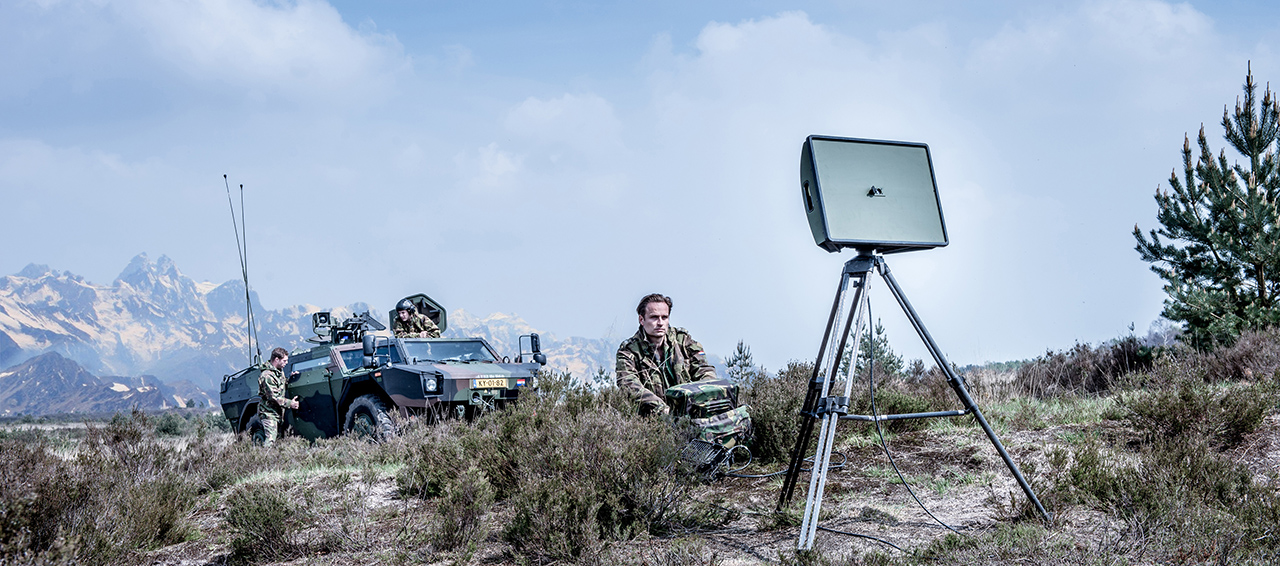
\includegraphics[width=\textwidth]{radar}
\captionof{figure}{Le radar portable Squire de Thales Air Systems}

Il existe néanmoins certains drones construits en carbone pouvant être perméables à certaines ondes radars et ainsi indétectables par cette technologie. Cependant le "radar passif", radar exploitant les variations d'ondes électromagnétiques en milieu urbain, telles que les ondes de la TNT, pourrait être exploité en milieu urbain.



\section{Radiogoniométrie}

Parmi les moyens existants pour détecter un drone on peut citer la radiogoniométrie. Le principe de la radiogoniométrie est de mesurer la direction d'arrivée d'une onde électromagnétique polarisée incidente sur un réseau de capteur, par rapport à une direction de référence. Les radio-goniomètres sont donc des détecteurs passifs. 

La radiogoniométrie possède de nombreuses applications. Cependant, en interception, la radiogoniométrie permet de localiser un émetteur inconnu soit en employant plusieurs récepteurs en des positions différentes, soit par calcul en fonction de la cinématique propre du récepteur. 

On distingue deux types de goniomètres: les goniomètres à une dimension qui n'estiment que le gisement ou l'azimut, et les goniomètres à deux dimensions qui estiment le gisement ou azimut ainsi que l'élévation. 


Dans le cas d'une détection de drones, le radio-goniomètre réalise une écoute de l'environnement avec un balayage de fréquences. Lorsque le drone émettra avec la personne qui le guide on pourra ainsi le localiser précisément.

L'avantage principal de la radiogoniométrie est qu'il s'agit d'une méthode de détection passive. Elle est donc difficilement décelable et cela fait d'elle une technique fréquemment utilisée en guerre électronique. 

Seulement, la radiogoniométrie a des failles. En effet, il existe sur le marché des drones auto-pilotés qui n'émettent pas car ils chargent avant le début de leur vol leurs trajectoires. Ainsi il n'y a pas de communication avec un quelconque utilisateur, et donc il n'y a aucun signal émis. Il est donc impossible de les localiser à l'aide de cette technique.





\section{Synthèse}

Une solution technique idéale couplerait l'ensemble des méthodes décrites ci-dessus pour pouvoir parer à toute éventualité. Une analyse des solutions présentes sur le marché ou en développement montre que les configurations les plus performantes associent au moins deux des modes de détection cités. On peut notamment citer le cas du système drone-detector \cite{dronedetector}.

Néanmoins nous avons choisi pour ce projet de nous concentrer, dans un premier temps, sur une détection uniquement à base de radiogoniométrie.

Les raisons de ce choix sont les suivantes : Dans un premier temps, pour pouvoir réaliser un prototype fonctionnel il est plus aisé de se baser sur la radiogoniométrie compte tenu du matériel à notre disposition. Dans un second temps, notre équipe a choisi de se concentrer sur la détection de drones de loisir disponibles dans le commerce. Selon la réglementation ces drones doivent maintenir un lien radio avec un pilote qui doit être en mesure de reprendre le contrôle du drone à tout instant. Il y a donc une liaison permanente qui peut être exploitée par le système.




% Ici il va falloir préciser plusieurs choses sur pourquoi ce choix. Notamment en précisant qu'on suppose que les drones respectent la réglementation, etc... 



%%% Local Variables: 
%%% mode: latex
%%% TeX-master: "rapport_analyse"
%%% End: 
